\hypertarget{defect_8cpp}{\section{defect.\-cpp \-File \-Reference}
\label{dd/def/defect_8cpp}\index{defect.\-cpp@{defect.\-cpp}}
}


\-Definition of member functions of the \hyperlink{classDefect}{\-Defect} class.  


{\ttfamily \#include \char`\"{}defect.\-h\char`\"{}}\*
\-Include dependency graph for defect.\-cpp\-:
\nopagebreak
\begin{figure}[H]
\begin{center}
\leavevmode
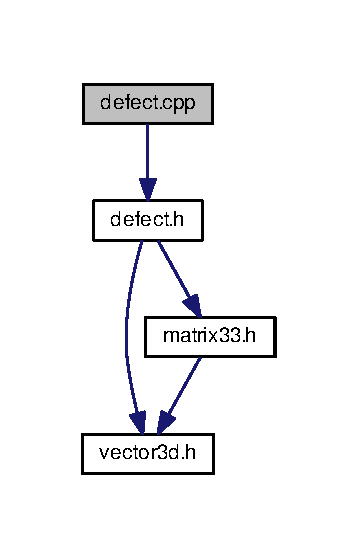
\includegraphics[width=188pt]{dd/dcf/defect_8cpp__incl}
\end{center}
\end{figure}


\subsection{\-Detailed \-Description}
\-Definition of member functions of the \hyperlink{classDefect}{\-Defect} class. \begin{DoxyAuthor}{\-Author}
\-Adhish \-Majumdar 
\end{DoxyAuthor}
\begin{DoxyVersion}{\-Version}
0.\-0 
\end{DoxyVersion}
\begin{DoxyDate}{\-Date}
22/04/2013
\end{DoxyDate}
\-This file defines the member functions of the \hyperlink{classDefect}{\-Defect} class representing a single defect in the simulation. 

\-Definition in file \hyperlink{defect_8cpp_source}{defect.\-cpp}.

